\chapter{Lernfeld 5: Software zur Verwaltung von Daten anpassen}

\textbf{Die Schülerinnen und Schüler verfügen über die Kompetenz, Informationen mittels
    Daten abzubilden, diese Daten zu verwalten und dazu Software anzupassen.}

Die Schülerinnen und Schüler informieren sich innerhalb eines Projektes über die Abbildung
von Informationen mittels Daten. Dabei \textbf{analysieren} sie Daten hinsichtlich Herkunft, Art,
Verfügbarkeit, Datenschutz, Datensicherheit und Speicheranforderung und berücksichtigen
Datenformate und Speicherlösungen.

Sie \textbf{planen} die Anpassung einer Anwendung zur Verwaltung der Datenbestände und entwickeln Testfälle. Dabei \textbf{entscheiden} sie sich für ein Vorgehen.

Die Schülerinnen und Schüler \textbf{implementieren} die Anpassung der Anwendung, auch im
Team und erstellen eine Softwaredokumentation.

Sie testen die Funktion der Anwendung und \textbf{beurteilen} deren Eignung zur Bewältigung der
gestellten Anforderungen.

Sie \textbf{evaluieren} den Prozess der Softwareentwicklung.

% Schreibtischtest

\section{UML (Unified Modeling Language)}

\begin{figure}[H]
    \centering
    \includesvg[width=\textwidth,inkscapelatex=false]{figures/UML.drawio.svg}
    \caption{Hierarchie UML Diagramme}
\end{figure}
\FloatBarrier

\subsection{Klassendiagramm}

\subsubsection{Elemente}

\begin{figure}[H]
    \centering
    \includesvg[width=0.5\textwidth,inkscapelatex=false]{chapter/lernfeld5/figures/simple_class.drawio.svg}
    \caption{Einfache Klasse}
\end{figure}
\FloatBarrier

Eine Klasse kann um Attribute erweitert werden. Dabei unterscheidet man zwischen Instanzattributen, welche Eigenschaften eines Objekts sind und zu Laufzeit gebildet werden, und Klassenattributen, welche Eigenschaften der Klassen und aller Instanzen der Klasse, aber unabhängig von diesen Instanzen sind. Klassenattribute werden unterstrichen dargestellt.

Es gilt generell: [Sichtbarkeit] [/] \textbf{Name} [:Typ] [Multiplizität] [=Vorgabewert] [\{Eigenschaft\}]

\begin{itemize}
    \item Sichtbarkeit
          \subitem +: public
          \subitem \#: protected
          \subitem -: private
          \subitem ~: package
    \item /: Aus anderen Werten ableitbar
    \item Multiplizität: Anzahl der Datenelemente mit [Untergrenze..Obergrenze], wobei * für beliebig viele steht
    \item {Eigenschaft}:
          \subitem {id}
          \subitem {readOnly}
          \subitem {subsets <Attribut>}
          \subitem {union <Attribut>}: Menge aller Teilmengen (subsets)
          \subitem {redefines <Attribut>}
          \subitem {ordered}: sortiert und eindeutige Werte
          \subitem {seq} | {sequence}: sortiert
          \subitem {unique}: eindeutige Werte
          \subitem {nonunique}
          \subitem {composite}
\end{itemize}

Desweiteren können Klassen um Operationen (Methoden) erweitert werden. Auch hier gibt es Objekt- und Klassenoperationen mit gleicher Notation und überschneidenden Merkmalen.

Es gilt generell: [Sichtbarkeit] \textbf{Name} ([Parameterliste]) [:Rückgabetyp] [Multiplizität] [\{Eigenschaft\}]

Für Parameter gilt generell: [Übergabemodus] \textbf{Name} :Typ [Multiplizität] [=Vorgabewert] [\{Eigenschaft\}]

Der Übergabemodus ist entweder "in" (default) für Parameter, welche von der Operation nur gelesen werden dürfen, "out" oder "return" für reine Ausgaben und "inout" für Parameter, welche sowohl gelesen als auch geschrieben werden dürfen.

Ähnlich mancher Programmiersprachen können Operationen überladen werden.

\subsection{Objektdiagramm}

\subsection{Kompositionsdiagramm}

\subsection{Komponentendiagramm}

\subsection{Verteilungsdiagramm}

\subsection{Paketdiagramm}

\subsection{Use-Case-Diagramm}

\begin{figure}[H]
    \centering
    \includesvg[width=0.3\textwidth,inkscapelatex=false]{chapter/lernfeld5/figures/system_boundary.drawio.svg}
    \caption{Systemgrenze}
\end{figure}
\FloatBarrier

\begin{figure}[H]
    \centering
    \includesvg[width=0.05\textwidth,inkscapelatex=false]{chapter/lernfeld5/figures/actor.drawio.svg}
    \caption{Akteur}
\end{figure}
\FloatBarrier

Alternative Darstellung eines Akteurs ist z.B. ein Stereotyp und Name in einem Rechteck oder ein aussagekräftiges beliebiges Symbol für ein Akteur.

\subsection{Aktivitätsdiagramm}

\begin{figure}[H]
    \centering
    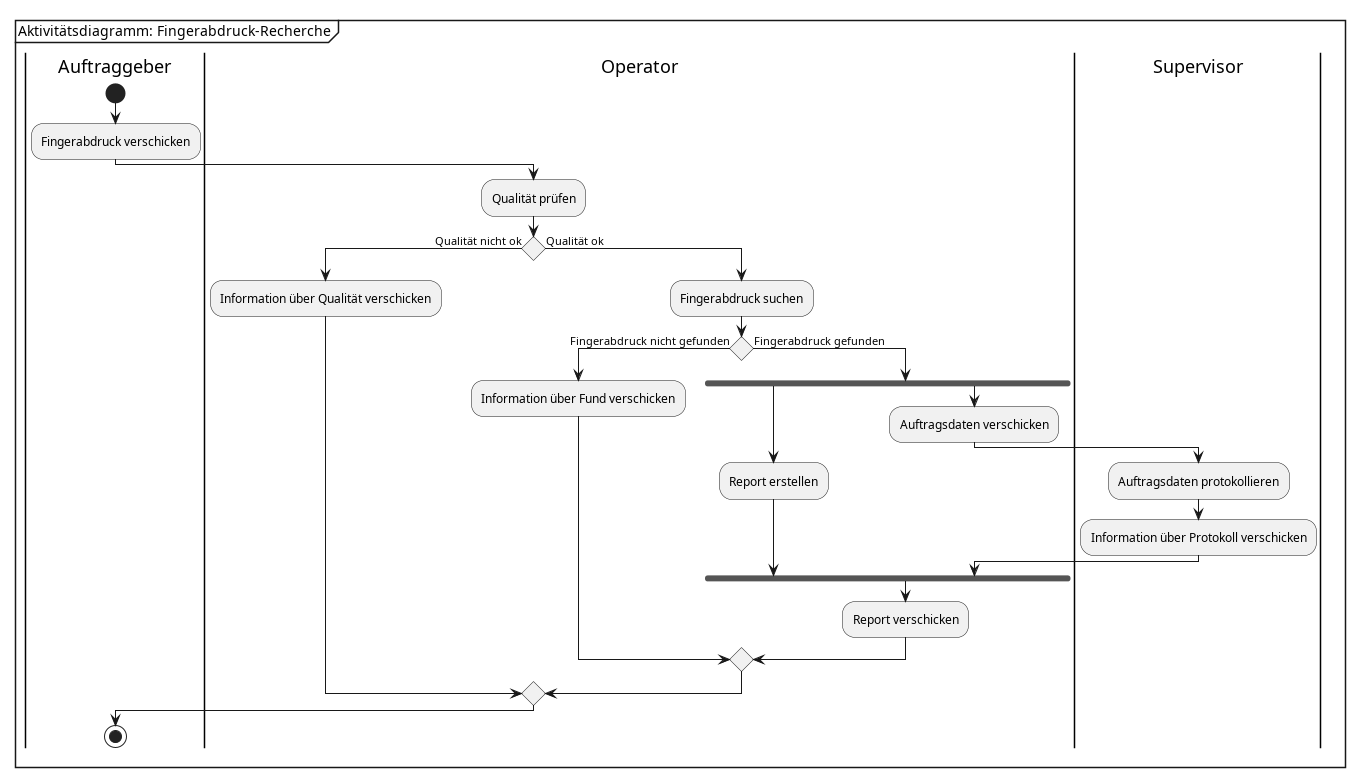
\includegraphics[width=\textwidth]{figures/activity.png}
    \caption{Beispiel Aktivitätsdiagramm}
\end{figure}

\subsection{Zustandsdiagramm}

\subsection{Sequenzdiagramm}

\subsection{Kommunikationsdiagramm}

\subsection{Zeitverlaufsdiagramm}

\subsection{Interaktionsübersichtsdiagramm}

\subsection{Profildiagramm}

\section{Struktogramm}